\subsection{Examples}
Now we try to illustrate the procedure's workings with respect of two example. First example shows how the procedure conclude $unsat$ for a set of constraints which are unsatisfiable. And the second shows how the procedure finds a saturated configuration for a set of constraints which are satisfiable. Both the examples are taken from \cite{main-paper}.
\begin{description}			
	\item[Example 1:] The input constraints are: $ A = \phi$ and $S = \{ \texttt{len}(x) \approx
	\texttt{len}(y), x \not\approx \epsilon, y\not\approx \epsilon, z \not\approx \epsilon, \texttt{con}(x, l_1, z) \approx \texttt{con}(y, l_2, z)\}$, where $l_1$, $l_2$ are distinct constants of the same length.	

The procedure starts with $step\ 0$ by applying \texttt{Reset}. It tries to find conflicts by applying   \texttt{S-Conflict} and \texttt{A-Conflict}. Since the arithmetic constraint set $A$ is empty and there are no contradicting string constraints in $S$, $check\ for\ contradiction$ fails. 

The procedure tries the step $propagate$. For this example this step does not introduce any new constraint in $S$, as $A$ is empty. Now the procedure applies \texttt{Len} and \texttt{Len-Split} repeatedly as long as there is possible application. The application of these two splitting rules causes the branching of the derivation tree. However, all branches are closed by rule  \texttt{S-Conflict} expect one. This is shows in Figure as the left branches of each configuration. 

In this non closing configuration, the string equivalence classes are $\{x\}, \{y\}, \{z\}, \{l_1\}, \{l_2\}, \{\epsilon\},$ and $\{ \texttt{con}(x, l_1, z), \texttt{con}(y, l_2, z)\}$. Now the procedure goes on to compute normal forms by applying \texttt{N-Form2}, \texttt{F-Form2} and \texttt{N-Form1}.The flat forms  \texttt{F} $\texttt{con}(x, l_1, z) = (x, l_1, z)$ and \texttt{F} $\texttt{con}(y, l_2, z) = (y, l_2, z)$ are computed by \texttt{F-Form1}. Then \texttt{F-Unify} is applied to add the equality $x \approx y$ to $S$. This causes the procedure to restart, but with an extended constraints set. Which induces a new equivalence classes $ \{x, y\}, \{z\}, \{l_1\}, \{l_2\}, \{\epsilon\}$, and $\{\texttt{con}(x, l_1, z), \texttt{con}(y, l_2, z)\}$. After similar steps, the procedure reached a stage where it computes the flat forms $(x, l_1, z)$ and $(x, l_2, z)$ for the  corresponding equivalence class,
by choosing $x$ as representative of $y$. At this point the procedure applies rule \texttt{F-Unify} again. This introduces a new equality $l_1 \approx l_2$ to $S$ and eventually derives \texttt{unsat} with \texttt{S-Conflict}. That is the procedure ended up with a derivation tree where each branch is closed and conclude that the input constraints are unsatisfiable.  The resulting derivation tree is shown in figure .

\begin{figure}
	\centering
	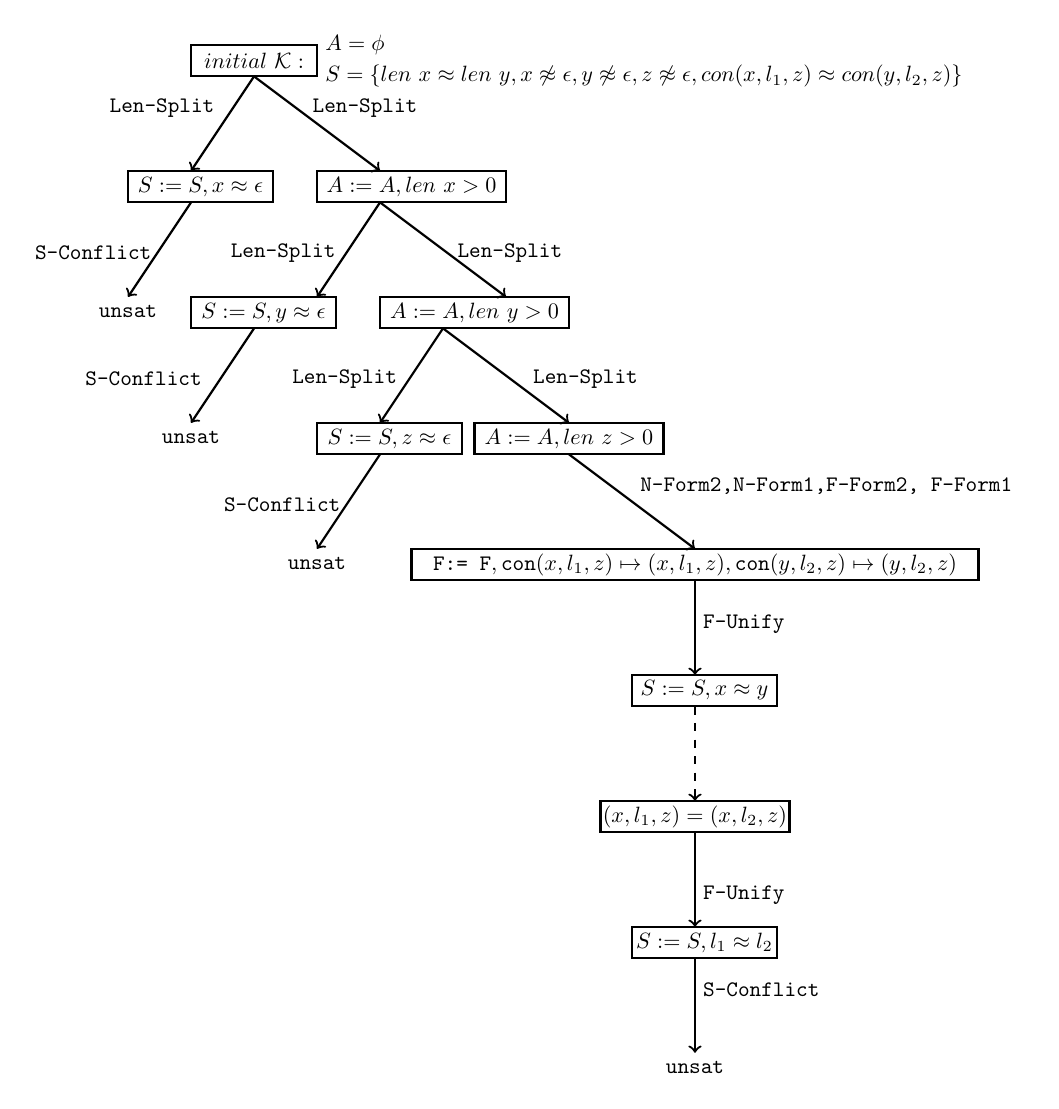
\begin{tikzpicture}[thick,scale=0.8, every node/.style={transform shape}]
	
	\node [right] at (3,20) { $ A=\phi $};
	\node [right] at (3,19.5) { $ S=\{  len \ x \approx len \ y, x \not\approx \epsilon, y \not\approx \epsilon,
		z \not\approx \epsilon, con (x, l_1,z) \approx con (y, l_2, z)\} $}; 
	 
    \draw (1,20) rectangle (3,19.5) node[pos=.5] {$ initial \ \mathcal{K}:$};
	
	\draw [->] (2,19.5) -- (1,18);
	\node [left] at (1.5,19) {$\texttt{Len-Split}$};
	
	\draw [->] (2,19.5) -- (4,18);
	\node [right] at (2.8,19) {$\texttt{Len-Split}$};
	
	
	\draw (0,18) rectangle (2.3,17.5) node[pos=.5] {$S:=S, x\approx \epsilon$};
	\node [rectangle, below] at (1,18) {};
	
	
	\draw (3,18) rectangle (6,17.5) node[pos=.5] {$A:=A, len \ x  > 0$};
	\node [rectangle, below] at (4,18) {};
	
	\draw [->] (1,17.5) -- (0,16);
	\node [left] at (0.5,16.7) {$\texttt{S-Conflict}$};
	
	\draw [->] (4,17.5) -- (3,16);
	\node [right] at (1.5,16.7) {$\texttt{Len-Split}$};
	\draw [->] (4,17.5) -- (6,16);
	\node [right] at (5.1,16.7) {$\texttt{Len-Split}$};
	
	\node [below] at (0,16) {$\texttt{unsat}$};
	\draw (1,16) rectangle (3.3,15.5) node[pos=.5] {$S:=S, y\approx \epsilon$};
	\node [below] at (2,16) {};
	\draw (4,16) rectangle (7,15.5) node[pos=.5] {$A:=A, len \ y  > 0$};
	\node [below] at (5,16) {};
	
	\draw [->] (2,15.5) -- (1,14);
	\node [left] at (1.3,14.7) {$\texttt{S-Conflict}$};
	\draw [->] (5,15.5) -- (4,14);
	\node [left] at (4.4,14.7) {$\texttt{Len-Split}$};	
	\draw [->] (5,15.5) -- (7,14);
	\node [right] at (6.3,14.7) {$\texttt{Len-Split}$};
	
	
	\node [below] at (1,14) {$\texttt{unsat}$};
	\draw (3,14) rectangle (5.3,13.5) node[pos=.5] {$S:=S, z\approx \epsilon$};
	\node [below] at (4,14) {};
	\draw (5.5,14) rectangle (8.5,13.5) node[pos=.5] {$A:=A, len \ z  > 0$};
	\node [below] at (7,14) {};


	\draw [->] (4,13.5) -- (3,12);
	\node [left] at (3.5,12.7) {$\texttt{S-Conflict}$};
	\draw [->] (7,13.5) -- (9,12);
    \node [right] at (8,13) {$\texttt{N-Form2,N-Form1,F-Form2, F-Form1 }$};
    

	
	\node [below] at (3,12) {$\texttt{unsat}$};
	\draw (4.5,12) rectangle (13.5,11.5) node[pos=.5] {$\texttt{F:= F},\texttt{con}(x,l_1,z)\mapsto (x,l_1,z),\texttt{con}(y,l_2,z)\mapsto(y,l_2,z)$};
	\node [below] at (9,12) {};
	
	\draw [->] (9,11.5) -- (9,10);
	\node [right] at (9,10.8) {$\texttt{F-Unify}$};
	
	\draw (8,10) rectangle (10.3,9.5) node[pos=.5] {$S:=S, x\approx y$};
	\node [below] at (9,10) {};
	
	\draw [dashed,->] (9,9.5) -- (9,8);
	
	\draw (7.5,8) rectangle (10.5,7.5) node[pos=.5] {$( x, l_1, z ) = (x, l_2,z)$};
	\node [below] at (9,8) {};
	
	\draw [->] (9,7.5) -- (9,6);
	\node [right] at (9,6.5) {$\texttt{F-Unify}$};
	
	\draw (8,6) rectangle (10.3,5.5) node[pos=.5] {$S:=S, l_1 \approx l_2$};
	\node [below] at (9,6) {};
	
	\draw [->] (9,5.5) -- (9,4);
	\node [right] at (9,5) {$\texttt{S-Conflict}$};
	
	\node [below] at (9,4) {$\texttt{unsat}$};
	
	
	
	
	
	
	\end{tikzpicture}
	\caption{The derivation tree for example 1. Here $l_1, l_2 $ are distinct constants of same length.}
\end{figure}	


	
	
\end{description}
\begin{description}			
	\item[Example 2:] The input constraints are: $ A = \phi$ and $S = \{ \texttt{len}(x) \approx
	\texttt{len}(y), x \not\approx \epsilon, z \not\approx \epsilon, \texttt{con}(x, l_1, z) \not\approx \texttt{con}(y, l_2, z)\}$, with $l_1$, $l_2$ are distinct constants of the same length.
	
	
	Similar to the previous example, the procedure reaches a configuration where the string equivalence classes are $ \{x\}, \{y\}, \{z\}, \{l_1\}, \{l_2\}, \{\epsilon\},\{ \texttt{con}(x, l_1, z)\}$ and,$\{\texttt{con}(y, l_2, z)\}$.
	In this case, the procedure attempts to partition the the equivalence classes into buckets. It fails to create the full partition, as rule \texttt{D-Base}  nor rule \texttt{D-Add} is applicable to $[y]$ because of $S \models \texttt{len} \ x \approx \texttt{len} \ y$ and  $x \not\approx y \not\in \mathcal{C}(S)$.  
	
	In such a case the procedure tries to guess by applying rule \texttt{S-Split} to $x$ and $y$. It case two branches in the derivation tree, one for $x \approx y$ and another for $x \not\approx y$.  
		
	After similar steps as in previous example, the procedure can derive a configuration where the string equivalence classes are $ \{x\}, \{y\}, \{z\}, \{l_1\}, \{l_2\}, \{\epsilon\},\{ \texttt{con}(x, l_1, z)\}$ and,$\{\texttt{con}(y, l_2, z)\}$. After computing normal forms for these classes, it attempts to	construct a partition \texttt{B} of them into buckets. However, notice that if it adds {[x]},say, to \texttt{B} using \texttt{D-Base}, then neither \texttt{D-Base} (since $S \models \texttt{len} \ x \approx \texttt{len} \ y$) nor \texttt{D-Add} (since $x \not\approx y \not\in \mathcal{C}(S)$ ) is applicable to $[y]$. So it applies \texttt{S-Split} to $x$ and $y$. In the branch where $ x \approx y$, the procedure subsequently restarts as new constraints are introduced to $S$. Eventually the procedure computes normal forms and succeeds in making a full partition of \texttt{B}. The procedure places $[\texttt{con}(x, l_1, z)]$ and $[\texttt{con}(y, l_2, z)]$ into the same bucket using \texttt{D-Add}, which applies because their corresponding normal forms are $(x, l_1, z)$ and $(x, l_2, z)$ respectively. Any further rule applications lead to branches with  a saturated configuration. Thus the procedure concludes that the problem is satisfiable. For each of the branches with saturated configuration satisfying models can be generated.
\end{description}
Here in this section we have tried to explore the inner working of the decision procedure. According to the authors \cite{main-paper}, the presented version the procedure is a simplified one. The procedure and derivation rules, which are implemented as part of cvc4 is much more complex and elaborate.